\chapter{Потенциометры}

\newthought{Потенциометр}\marginnote{\allcaps{ПОТЕНЦИОМЕТР}} --- регулируемый делитель напряжения, представляющий собой, как правило, резистор с подвижным отводным контактом (движком). Он предназначен для получения электрического сигнала, функционально зависящего от углового или поступательного перемещения токосъемного элемента (движка с контактами). При соответствующем включении он может быть использован и как резистор с переменным сопротивлением. Это определение относится к электромеханическим переменным резисторам.

Вследствие относительной простоты конструкции и широты реализуемых функций потенциометры получили значительное распространение в приборостроении: 
\begin{itemize}
	\item в измерительных системах их используют как первичные преобразователи механического перемещения в электрическое напряжение;
	\item в автоматических системах потенциометры часто применяют как элементы обратной связи;
	\item в вычислительной технике --- для реализации функциональных аналоговых зависимостей.
\end{itemize}

В зависимости от материала резистивного элемента и конструкции потенциометра различают: проволочные, пленочные, пластиковые, фотоэлектрические, жидкостные и цифровые потенциометры, которые являются альтернативой электромеханическим переменным резисторам.

\section{Проволочные потенциометры}

Простейший по конструкции проволочный потенциометр (рис.~\ref{pic:8potentiometer}~а) представляет собой каркас~1 постоянного или переменного поперечного сечения, выполненный из токонепроводящего материала или из алюминиевого сплава с электроизоляцией. На каркас намотана проволока~5 (резистивный элемент), от которой в точках А и В сделаны два отвода~6. По зачищенной от изоляции поверхности проволоки (контактной дорожке) перемещается подвижный контакт~4, связанный с движком~2 (токосъемник). От подвижного контакта~4 сделан отвод~3. Полная рабочая длина потенциометра~l0 меньше длины намотки~$ l $. Это делают для того, чтобы не происходило размыкания цепи и повреждения контакта~4 при выходе движка за расчетные пределы его перемещения.

\begin{figure}[h!]
	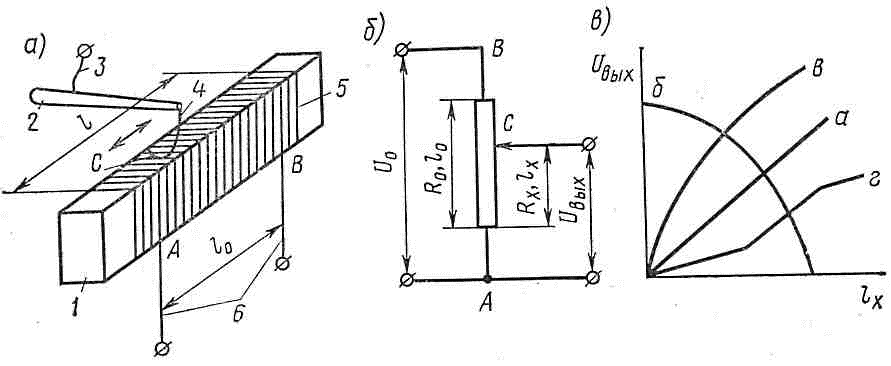
\includegraphics[width=1\textwidth]{8potentiometer.png}
	\caption[Проволочный потенциометр]{ Проволочный потенциометр: а -- конструкция, б -- электрическая схема, в -- характеристика }
	\label{pic:8potentiometer}
\end{figure}

\begin{figure}[h!]
	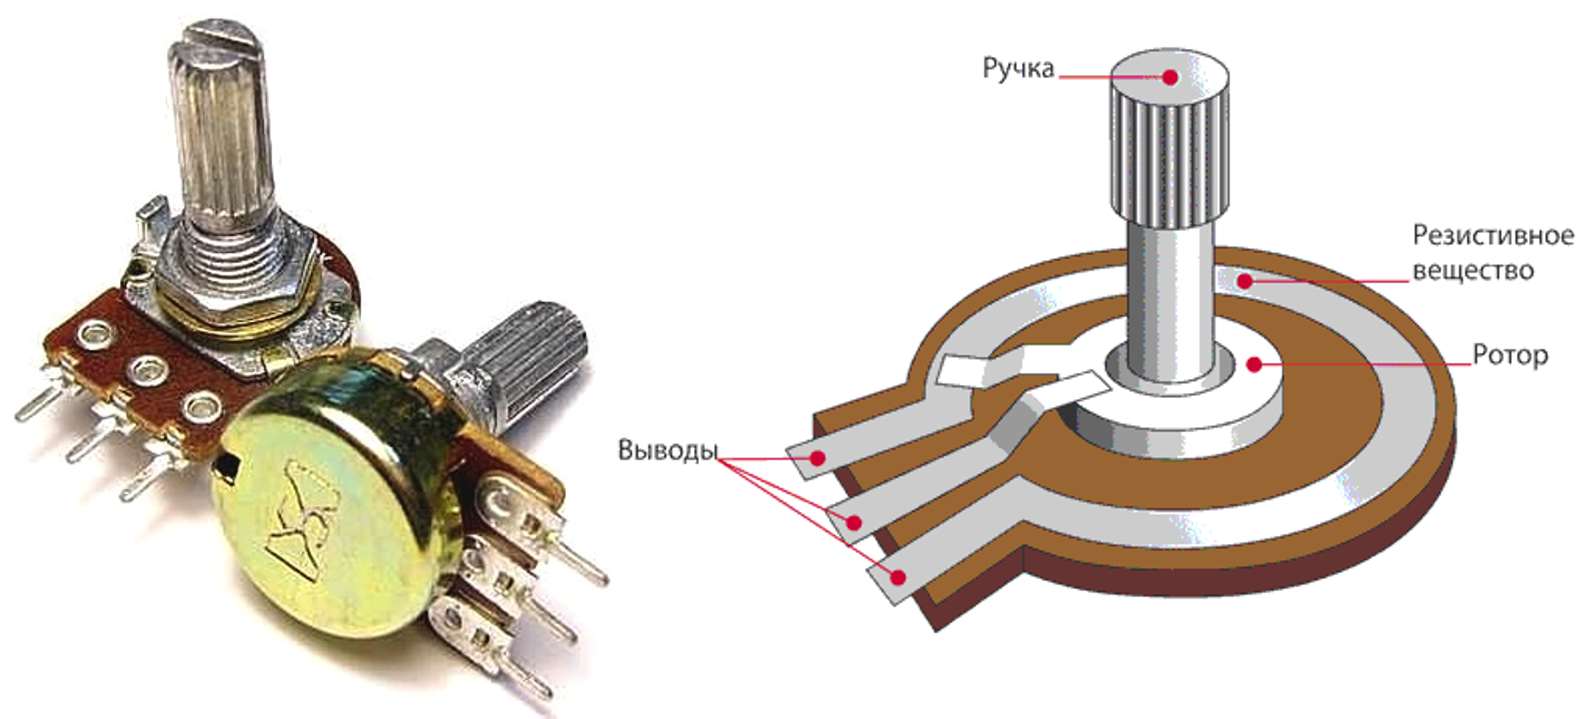
\includegraphics[width=1\textwidth]{8potentiometer1.png}
	\caption{ Потенциометр }
	\label{pic:8potentiometer1}
\end{figure}

Электрическая схема потенциометра показана на рис.~\ref{pic:8potentiometer}~б. Входное напряжение $ U_0 $ (напряжение питания) подводится к точкам А и В, а выходное $ U_\text{вых} $ снимается с участка между точками А (или В) и С (скользящий контакт). Сопротивление $ R_x $ потенциометра связано с перемещением движка $ l_x $ зависимостью $ R_x = \dfrac{R_0l_x}{l_0} $, где $ R_0 $~-- полное сопротивление потенциометра. Тогда при ненагруженном потенциометре
\[ U_\text{вых} = \dfrac{U_0 R_x}{R_0} = \dfrac{U_0 l_x}{l_0} \]

Зависимость $ U_\text{вых} = f(l_x) $ называется характеристикой потенциометра. Если приращение сопротивления на единицу перемещения движка постоянно, то потенциометр имеет линейную характеристику (кривая а на рис.~\ref{pic:8potentiometer}~в). (Если $ \dfrac{\Delta l_x}{\Delta U_\text{вых}} = const $, то потенциометр линейный). Если же сопротивление потенциометра нелинейно зависит от $ l_x $, т.е. $ R_x = R_0 f(l_x/l_0) $, то и $ U_\text{вых} = U_0 f(l_x/l_0) $. Такие потенциометры называются функциональными (кривые б, в и г на рис.~\ref{pic:8potentiometer}~в).

По типу перемещения движка потенциометры разделяют на потенциометры с поступательным (рис.~\ref{pic:8potentiometer}~а) и вращательным (рис.~\ref{pic:8type}~а) перемещением движка. В многооборотных потенциометрах (рис.~\ref{pic:8type}~б) подвижный контакт~1, имеющий форму ролика, совершает винтовое перемещение по каркасу~2, выполненному в виде спирали из медного стержня диаметром 1$ \ldots $2~мм. На каркас намотан тонкий резистивный провод. Существуют и другие схемы многооборотных потенциометров. Многооборотные потенциометры позволяют получить при небольших габаритах большую рабочую длину резистивного элемента.

\begin{figure}[h!]

	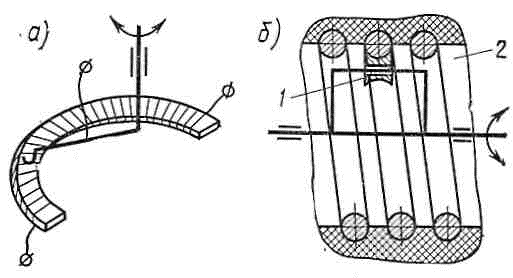
\includegraphics[width=0.8\textwidth]{8type.png}
	\label{pic:8type}
\end{figure}

Важным элементом конструкции потенциометра является движок с контактом. Движок должен обладать малой инерционностью и большой жесткостью. 

\newthought{Пленочный потенциометр}\marginnote{\allcaps{ПЛЁНОЧНЫЙ\break ПОТЕНЦИОМЕТР}} состоит из тонкой резистивной металлической или угольной пленки с выводами выходного напряжения на концах и скользящего контакта. 
Резистивный элемент металлопленочного потенциометра представляет собой тонкий слой высокоомного металла толщиной 2-3~мкм, нанесенного на стеклянную пластинку.

Он характеризуется бесконечной разрешающей способностью, высокой точностью и надежностью. 
Чтобы получить требуемую величину, необходима очень малая (до прозрачности) толщина металлической пленки, что лимитирует срок ее службы и надежность. Углеродные пленки могут быть намного толще, так как углерод обладает высоким удельным сопротивлением. 
Кроме того, они характеризуются низким уровнем шумов, автоматической смазкой и устойчивостью против коррозии.

Разработаны потенциометры с металлокерамическим резистивным элементом и с пленками на основе проводящих пластиков.

Сопротивление металлопленочного потенциометра в отличие от проволочного не носит ступенчатого характера, вследствие чего исчезает витковая погрешность, уменьшение которой в проволочных потенциометрах имеет определенные пределы, особенно при малых номинальных значениях общего сопротивления. 

Фактически неограниченная разрешающая способность пленочных потенциометров обеспечивает бесконечное число положений контакта на резистивном элементе. Кроме того, момент вращения металлопленочных потенциометров меньше, чем у проволочных. 
Общее сопротивление таких потенциометров лежит в пределах от 100~Ом до 1~Мом, погрешность характеристики не превышает 0,5 \%. 
Металлоплёночные потенциометры применяются в приборах с потенциометрическими дистанционными передачами и следящими системами.

В пластиковых потенциометрах резистивный элемент выполняют из твердых токопроводящих пластмасс. Такие потенциометры отличает большая износостойкость.

\newthought{В фотопотенциометре}\marginnote{\allcaps{ФОТОПОТЕНЦИОМЕТР}} (рис.~\ref{pic:8photopotentiometer}~а) роль скользящего контакта выполняет световое пятно~2, перемещающееся по фотопроводнику~1, который соединяет между собой резистивный элемент~4, выполненный в виде тонкой полоски из металла с высоким сопротивлением и токосъемник~3, имеющий малую величину сопротивления. В месте, где световое пятно~2 падает на фотопроводник~1, создается токопроводящий мост между резистивным элементом~4 и токосъемником~3. Существуют различные способы применения фото потенциометров. 

На рис.~\ref{pic:8photopotentiometer}~б представлена схема использования фотопотенциометра~3 с подвижным источником света~1. Маска~2 в этом случае неподвижна. 
Существуют также конструкции, в которых подвижной является маска, а не источник света.

\begin{figure}[h!]
	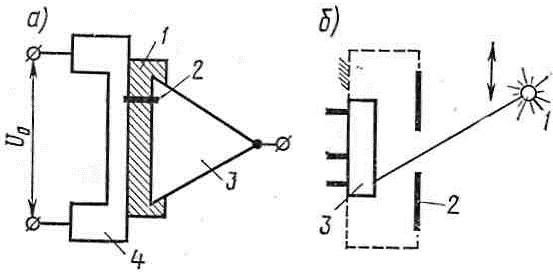
\includegraphics[width=0.6\textwidth]{8photopotentiometer.png}
	\caption{ Фотопотенциометр }
	\label{pic:8photopotentiometer}
\end{figure}

\newthought{Жидкостный потенциометр}\marginnote{\allcaps{ЖИДКОСТНЫЙ\break ПОТЕНЦИОМЕТР}} --- потенциометр, в котором в качестве резистивного элемента используется жидкость. 
Жидкостный потенциометр конструктивно представляет собой сосуд, заполненный токопроводящим электролитом. 
В сосуд введены два электрода~-- подвижный и неподвижный. 
При изменении расстояния между ними изменяется длина столба токопроводящего электролита, а, следовательно, и значение его электрического сопротивления.
Например, жидкостный потенциометр с линейным изменением сопротивления может иметь несколько электродов с вертикальным перемещением. 
Общее (входное) напряжение подводится на заземленный экран и не заземленный металлический электрод. 
Линейную и нелинейную функции можно воспроизвести, придав определенную форму электродам и экрану.

В потенциометре с вращающимся электродом общее напряжение подводится на две неподвижные лопасти, третья~-- подвижная лопасть служит выходным электродом. 
Вторым выходным электродом является вращающаяся лопасть. 
Таким образом, отпадает надобность в скользящих металлических контактах. 
Придав лопасти определенную форму, можно получить различные законы изменения сопротивления потенциометра как функции угла поворота его оси. Сопротивление жидкостных потенциометров зависит от электролита и составляет от нескольких сот Ом до нескольких МОм.

\section{Основные параметры и характеристики}

Потенциометр является электромеханическим устройством, и поэтому его характеристики могут быть разделены на:
\begin{itemize}
	\item электрические: полное сопротивление, мощность, предельное рабочее напряжение;
	\item механические: угловое или линейное перемещения движка, момент трогания.
\end{itemize}

Полное сопротивление $ R_0 $ потенциометра зависит от геометрических размеров и параметров (удельное электрическое сопротивление $ \rho $, размеры поперечного сечения) резистивного элемента~-- обмотки или покрытия. 
Значение $ R_0 $ снизу ограничивается допустимым нагревом потенциометра (при заданном напряжении $ U_0 $), а сверху~-- технологической возможностью изготовления проводника с малыми размерами поперечного сечения, а также сроком службы, так как тонкий проводник быстрее протирается подвижным контактом. 
Сопротивление потенциометра зависит от его температуры, которая определяется температурой окружающей среды и нагревом резистивного элемента, протекающим по нему током. 
Влияние температуры на $ R_0 $ объясняется зависимостью от температуры удельного сопротивления $ \rho $ материала резистивного элемента. 
Изменение геометрических размеров резистивного элемента и корпуса с изменением температуры сказывается значительно меньше.

Температурное изменение сопротивления потенциометра оценивается температурным коэффициентом сопротивления (ТКС) который представляет собой относительное изменение сопротивления потенциометра при изменении его температуры на 1~$ ^\circ $С. Среднее значение ТКС может быть определено отношением
\[\text{ТКС}_\text{среднее} = \dfrac{\Delta R}{R_0 \Delta t},\]
где $ \Delta R $ -- алгебраическая разность сопротивлений на границах интервала температур $ \Delta t $, $ R_0 $~-- сопротивление потенциометра при нормальной температуре.

У проволочных потенциометров $ \text{ТКС}_\text{мин} - 0,1\ldots2*10^{-4} \dfrac{1}{^\circ C} $, у пленочных и пластиковых он больше.

Важной характеристикой потенциометра является разрешающая способность. 
В проволочных потенциометрах равномерное перемещение подвижного контакта приводит к дискретному изменению $ U_\text{вых} $ (рис.~\ref{pic:8resolution}), так как контакт перемещается не по длине провода, а переходит с одного витка на другой. 

\begin{figure}[h!]	
	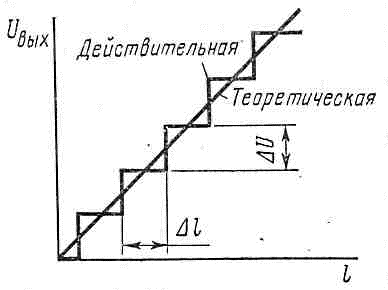
\includegraphics[width=0.6\textwidth]{8resolution.png}
	\caption{ Действительная и теоретическая характеристики потенциометра }
	\label{pic:8resolution}
\end{figure}

Значение скачков напряжения $ \Delta U $, характеризующее разрешающую способность, обратно пропорционально числу витков $ \omega $ обмотки: $ \Delta U = \dfrac{U_0}{\omega} $ (обратная $ \Delta U $ величина~-- количественная мера разрешающей способности). Разрешающая способность связана с так называемой витковой погрешностью $ \delta_\text{в} $, определяемой как наибольшее отклонение, вызванное дискретностью изменения $ U_\text{вых} $, от теоретической характеристики. Так как это отклонение равно $ \Delta U/2 $ (рис.~\ref{pic:8resolution}), то витковая погрешность
\[ \delta_\text{в} = \dfrac{\Delta U}{2U_0} 100 = \dfrac{100}{2\omega}. \]

Уменьшить витковую погрешность можно увеличением числа витков. Разрешающая способность пластиковых потенциометров, объясняющаяся зернистостью материала, несравненно больше, чем у проволочных, а у металлопленочных потенциометров разрешающая способность бесконечна.

Под механической разрешающей способностью понимается наименьшее изменение положения движка, которое приводит к изменению $ U_\text{вых} $. Наибольшее его значение (без учета промежуточных скачков) $ \Delta l = l_0/\omega $.

На характеристику потенциометра большое влияние оказывает сопротивление нагрузки $ R_\text{н} $. Выражение $ U_\text{вых} = \dfrac{U_0 R_x}{R_0} = \dfrac{U_0 l_x}{l_0} $ справедливо только при бесконечно большом сопротивлении нагрузки (при разрыве выходной цепи, $ R_\text{н} = \infty $). 

\begin{figure}[h!]
	\begin{center}
		\caption{ Схема включения потенциометра }
		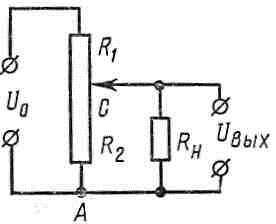
\includegraphics[width=0.4\textwidth]{8nagruzka.png}
		\label{pic:8nagruzka}
	\end{center}
\end{figure}

Обозначим \textsc{коэффициент нагрузки} $ k = \dfrac{R_\text{н}}{R_0} $ и \textsc{передаточный коэффициент} $ \alpha = \dfrac{R_2}{R_0} $:
\[ U_\text{вых} = \dfrac{\alpha U_0}{1+\dfrac{\alpha (1-\alpha)}{k}} \]

Из этого выражения следует, что чем меньше $ R_\text{н} $, тем больше действительная характеристика отличается от идеальной 
\[U_\text{вых} = \alpha U_0,\]
которая получается при $ R_\text{н} = \infty (k = \infty) $. Абсолютное значение отклонения:
\[ \Delta U_\text{вых} = \alpha U_0 - \dfrac{\alpha U_0}{1 + \dfrac{\alpha}{k}(1-\alpha)} = \dfrac{\alpha^2 (1-\alpha) U_0}{k+\alpha(1-\alpha)}.\]

На рис.~\ref{pic:8error} показаны зависимости относительной погрешности $ \dfrac{\Delta U_\text{вых}}{U_0} $ от передаточного коэффициента $ \alpha $ при различных значениях $ k $.

\begin{figure}[h!]
	\begin{center}
		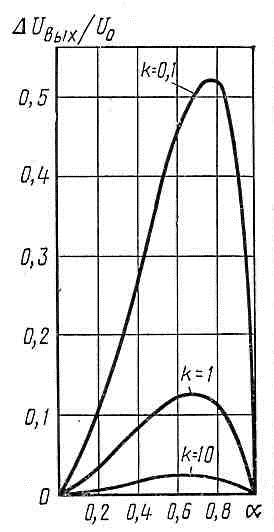
\includegraphics[width=0.4\textwidth]{8error.png}
		\label{pic:8error}
		\caption{ Зависимость относительной погрешности от передаточного коэффициента $ \alpha $ при различных $ k $}
	\end{center}
\end{figure}

Значение $ R_\text{н} $ при проектировании потенциометра обычно известно. Поэтому для увеличения $ k $ необходимо уменьшать $ R_0 $, но чрезмерное снижение $ R_0 $ приводит к увеличению нагрева потенциометра и уменьшению разрешающей способности. Иногда для устранения влияния нагрузки линейный потенциометр проектируют так, чтобы при холостом ходе он имел такую функциональную характеристику, которая при включении потенциометра на заданную нагрузку становится линейной. Для снижения влияния нагрузки используют также добавочные или шунтирующие резисторы. На рис.~\ref{pic:8resistor}~а показана схема включения потенциометра с добавочным резистором.

\begin{figure}[h!]
	\begin{center}
		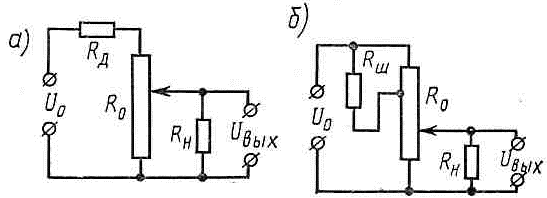
\includegraphics[width=0.8\textwidth]{8resistor.png}
		\caption{ Схемы включения потенциометра для устранения влияния нагрузки }
		\label{pic:8resistor}
	\end{center}
\end{figure}

При такой схеме включения для работы используется как бы только часть потенциометра с полным сопротивлением, равным $ R_\text{д} + R_0 $. Максимальное значение относительной погрешности $ \Delta U_\text{вых}/U_0 $ при $ R_\text{д}=0,5R_0 $ и $ k > 10 $ в четыре раза меньше, чем у некомпенсированного потенциометра. В схеме на рис.~\ref{pic:8resistor}~б предусматривается использование шунта между источником питания и обмоткой потенциометра. Наиболее эффективно (при $ k > 10 $) подсоединение шунта к обмотке в точке $ \alpha = 0,74 $. Шунт должен иметь сопротивление $ R_\text{ш} = 0,31 R_\text{н} $. При этих условиях максимальное значение относительной погрешности в семь раз меньше, чем у некомпенсированного потенциометра.

\textsc{Номинальная мощность рассеяния} --- это мощность, которая может длительное время рассеиваться потенциометром в заданных условиях эксплуатации при сохранении параметров в установленных пределах. Мощность рассеяния потенциометра определяется его конструкцией и свойствами используемых материалов. В режиме холостого хода ($ R_\text{н} = \infty $)   
\[ P_\text{ном} = I^2\,R_0 = \dfrac{U_0^2}{R_0}\]

При $ R_\text{н} \neq \infty $ мощность рассеяния (ее называют действительной) зависит от коэффициента нагрузки и схемы включения потенциометра. При известных значениях $ P_\text{ном} $ и $ R_0 $ из выражения для $ P_\text{ном} $ определяем значение рабочего напряжения питания $ U_\text{раб} \leq \sqrt{R_0\,P_\text{ном}} $. Это выражение ограничивает напряжение питания из условия предупреждения перегрева при использовании потенциометра в рабочем диапазоне температур. При повышении температуры окружающей среды $ U_\text{раб} $ должно быть уменьшено. Одновременно следует отметить, что $ U_\text{раб} $ должно быть меньше значения пробивного напряжения между резистивным элементом (а также его выводами) и корпусом.

Наиболее важными механическими характеристиками потенциометра являются \textit{допустимая скорость перемещения движка} и \textit{момент трогания}. 

\textsc{Допустимая скорость движка} определяется возможностью отрыва подвижного контакта от резистивного элемента при так называемой критической скорости его перемещения.

\textsc{Момент трогания} --- это минимальный момент, который необходимо приложить к оси движка для ее поворота. 

\textsc{Износоустойчивость потенциометра} оценивается наибольшим числом полных перемещений движка, при котором параметры потенциометра не выходят за установленные пределы. Износоустойчивость зависит от скорости перемещения движка, режимов и условий эксплуатации, конструкции подвижной системы, но наиболее значительное влияние оказывают контактное давление и механические свойства материалов контакта и резистивного элемента. 

Износоустойчивость можно существенно увеличить уменьшением значения контактного усилия. 
Это одновременно приводит к снижению момента трогания. Но в то же время уменьшаются стойкость контакта к вибрациям и ударам, допустимая скорость перемещения движка и надежность потенциометра. 

Потенциометры являются одной из наименее надежных частей устройств, в которых их применяют. 
Если же учесть большую применяемость потенциометров, то становится ясным, сколь большое внимание при проектировании следует обращать на вопросы повышения их надежности. 
Основными причинами отказов потенциометров являются износ, ненадежность контакта, механическое разрушение резистивного элемента. 
Особую опасность представляют временные отказы в виде кратковременного разрыва цепи. 
Это может произойти вследствие отскакивания контакта или попадания грязи, пыли и окисленных продуктов износа между контактом и резистивным элементом. 

В микроэлектронике в основном применяются цифровые потенциометры (ЦП). 
Большая часть регулировок в процессе производства и при обслуживании микроэлектронной аппаратуры возлагается на микропроцессоры. 
Такой подход имеет очевидные преимущества, а реализовать его помогают цифровые потенциометры (ЦП). 
В микроэлектронной аппаратуре стараются не устанавливать какие-либо механические подстроечные элементы.  
Причин этому несколько: большие затраты на реализацию ручного процесса регулировки, низкая точность регулировки, невысокая надежность подстроечных элементов. 

\section{Цифровые потенциометры}

\textsc{Микропроцессор} --- процессор (устройство, отвечающее за выполнение арифметических, логических операций и операций управления, записанных в машинном коде), реализованный в виде одной микросхемы или комплекта из нескольких специализированных микросхем (в отличие от реализации процессора в виде электрической схемы на элементной базе общего назначения или в виде программной модели).

\textsc{Цифро-аналоговый преобразователь (ЦАП)}~--- устройство для преобразования цифрового (обычно двоичного) кода в аналоговый сигнал (ток, напряжение или заряд). Цифро-аналоговые преобразователи являются интерфейсом между дискретным цифровым миром и аналоговыми сигналами.

\textsc{Аналого-цифровой преобразователь (АЦП)} производит обратную операцию.

\textsc{Интерфейс} --- совокупность средств, методов и правил взаимодействия между элементами системы.

\textsc{Цифровые потенциометры} --- альтернатива электромеханическим переменным резисторам. Их применение позволяет придать новые свойства электронным устройствам при одновременном уменьшении массогабаритных показателей и повышении надежности. Практически каждая электронная схема содержит элементы, предназначенные для заводской подстройки характеристик или для оперативного управления ими пользователем аппаратуры. В подавляющем большинстве случаев для этих целей предназначены переменные резисторы, номенклатура которых весьма велика. Заменой электромеханическим резисторам с подвижным контактом, имеющим ограниченный ресурс, относительно большие габариты, требующим ручной установки в необходимое положение, становятся цифровые потенциометры (ЦП). Они тоже имеют свои ограничения по применению, однако при грамотном использовании способны заменить электромеханические устройства в подавляющем большинстве применений.

Цифровые потенциометры широко используются в персональных компьютерах, аппаратуре телекоммуникации, контроллерах, изделиях промышленного, бытового и автомобильного назначения. Цифровыми потенциометрами регулируется яркость и контрастность ЖКИ дисплеев, громкость и тон звучания акустической аппаратуры, организуется автоматическое регулирование усиления. Они представляют собой линейку из последовательно соединенных резисторов с управляемым положением токосъема посредством внешнего интерфейса. Закон зависимости значения сопротивления от положения «движка» может быть линейным, логарифмическим, а также программируемым пользователем.

К классу цифровых потенциометров можно отнести прецизионные резистивные делители с различным отношением сопротивлений и управляемые прецизионные делители напряжения. В корпусе микросхемы могут располагаться до шести цифровых потенциометров. 

Монолитное исполнение с цифровым регулированием позволяет уменьшить мощность потребления, улучшить массогабаритные и эксплуатационные характеристики. Цифровые потенциометры позволяют осуществлять регулировку и подстройку электронных схем подобно обычным регулируемым резисторам, реостатам и механическим потенциометрам. 

Структурная схема типичного цифрового потенциометра показана на рис.~\ref{pic:8scheme}.

\begin{figure}[h!]
	\begin{center}
		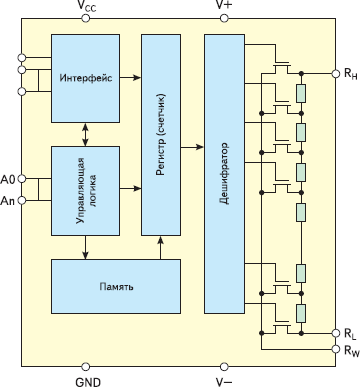
\includegraphics[width=0.7\textwidth]{8scheme.png}
		\caption{ Структурная схема цифрового потенциометра }
		\label{pic:8scheme}
	\end{center}
\end{figure}

Цепочка резисторов с отводами, коммутируемыми ключами, представляет собой собственно потенциометр с тремя выводами $ R_\text{H}, R_L $ и $ R_W $. Положение движка $ R_W $ определяется позицией замкнутого ключа. Ключи управляются регистром (счетчиком) через дешифратор. Состояние счетчика изменяется через интерфейс входными логическими сигналами либо непосредственно, либо считыванием установленной в энергонезависимой памяти позиции. Управляющая логика обеспечивает заданный режим работы. Конкретный тип ЦП в зависимости от своих функциональных возможностей может иметь как более простую, так и более сложную схему.

В ЦП отсутствует подвижный контакт к резистивному элементу, его функции выполняет набор электронных ключей, коммутирующий отводы от цепочки резисторов на вывод $ R_W $. В качестве ключей используются МОП-транзисторы, а сопротивление канала выступает в роли контактного сопротивления (сопротивления движка). 

Следующее отличие ЦП от электромеханических резисторов в дискретном характере изменения сопротивления. Поскольку резистивный элемент представляет собой цепочку резисторов с отводами, сопротивление изменяется скачками от ступени к ступени, а разрешающая способность зависит от количества ступеней, которых в различных моделях ЦП может быть от 8 до 1024. 

Принципиальное отличие ЦП от переменных резисторов в том, что напряжение на выводах ЦП не может быть больше регламентированного. Для большинства моделей это напряжение не может превышать напряжения питания. Подавляющее большинство ЦП предназначены для работы с однополярным источником питания напряжением 3-5 В, соответственно и потенциалы на выводах должны находиться в пределах 0–3(5) В. Это ограничивает область применения ЦП, но с учетом тенденции снижения питающего напряжения аппаратуры мест, в которых переменные резисторы не могут быть заменены ЦП, остается все меньше.

Обычные переменные резисторы после регулировки сохраняют свое положение. С ЦП все сложнее: достаточно выключить питание, как он <<забывает>> свое положение. При следующем включении питания ЦП устанавливается в определенное начальное положение, которое зависит от типа ЦП. Если в системе есть микропроцессор, то после включения питания он сразу может загрузить нужные коды, восстановив положение ЦП, найденное при регулировке. 

А если ЦП установлен в изделии, не имеющем микропроцессора или его вмешательство нежелательно? Для таких целей выпускается ряд типов ЦП со встроенной энергонезависимой памятью. Достаточно один раз настроить такой ЦП (кнопками или с помощью микропроцессора), как он запоминает положение и восстанавливает его при включении питания.

По сравнению с обычными переменными резисторами, ЦП имеют ряд преимуществ:
\begin{itemize}
	\item отсутствие подвижных механических частей; 
	\item высокая надежность; 
	\item нечувствительность к вибрациям; 
	\item нет проблем с контактом при работе на малых токах; 
	\item не требуется регулировочных отверстий для отвертки; 
	\item быстрый процесс настройки; 
	\item высокая точность регулировки; 
	\item корпуса микросхем более компактны, чем корпуса подстроечных резисторов; 
	\item стоимость цифровых потенциометров меньше стоимости качественных переменных резисторов. 
\end{itemize}

Существуют некоторые отличия цифровых потенциометров от обычных механических переменных резисторов, которые накладывают ограничения на их применение и в большинстве случаев являются недостатками. Далее при перечислении параметров ЦП видны их недостатки.

Важнейшим параметром ЦП\marginnote{\allcaps{ПАРАМЕТРЫ ЦП}} является количество коммутируемых отводов переменного резистора (количество шагов). Этот параметр определяет дискретность регулировки. Обычно количество шагов является степенью числа 2, но бывают ЦП и с другим количеством шагов, например 100. Наиболее распространены ЦП с количеством шагов от 32 до 256. 

Еще одним важным параметром ЦП, впрочем, как и обычного переменного резистора, является полное сопротивление. Наиболее распространены ЦП с полным сопротивлением 10, 50 и 100 кОм.

Среди других параметров ЦП необходимо отметить максимальное напряжение на выводах переменного резистора, сопротивление «щетки», максимальный допустимый ток, максимальную рассеиваемую мощность, шум, нелинейность и температурный коэффициент. Значения этих параметров у разных типов ЦП могут существенно отличаться, подробности можно найти в фирменной документации.

Пожалуй, самое главное отличие от переменных резисторов заключается в том, что ЦП нельзя включать в цепь, потенциал которой выходит за пределы допустимого напряжения на выводах переменного резистора. Чаще всего это напряжение не должно выходить за пределы напряжения питания ЦП. Для многих ЦП допустимый диапазон напряжений питания равен $ 0\ldots5 $~В, поэтому и использоваться они могут лишь в цепях с такими потенциалами. Некоторые типы ЦП допускают напряжение на выводах переменного резистора большее, чем напряжение питания. В то же время в измерительной аппаратуре часто используется напряжение питания $ \pm $15 В, что затрудняет применение там большинства ЦП. Дело в том, что производство ЦП подчиняется общей тенденции перехода на низкое напряжение питания $ \pm $5~В или даже $ \pm $3~В. 

Области применения ЦП\marginnote{\allcaps{ОБЛАСТИ\break ПРИМЕНЕНИЯ ЦП}} в настоящее время весьма разнообразны и их становится все больше в связи с появлением более совершенных ЦП. Вот некоторые из этих областей:
\begin{itemize}
	\item цифровая регулировка усиления; 
	\item реализация регулируемых источников опорного напряжения; 
	\item регулировка громкости в аудиосистемах; 
	\item регулировка смещения нуля в усилителях; 
	\item регулировка выходного напряжения стабилизаторов; 
	\item настройка измерительных мостов; 
	\item регулировка усиления, частоты настройки и добротности фильтров; 
	\item регулировка полной шкалы и смещения в усилителях датчиков; 
	\item регулировка частоты и скважности генераторов; 
	\item регулировка смещения pin-диодов в ВЧ-аттенюаторах; 
	\item регулировка контрастности ЖК-индикаторов. 
\end{itemize}

В настоящее время широко рекламируется возможность применения ЦП в качестве регуляторов громкости и тембра в аудиоаппаратуре. 
Однако обычные ЦП имеют для этого слишком маленький динамический диапазон и большие искажения. 
Для цифровых потенциометров остается лишь узкая ниша low-end применений, таких как регулировка громкости в сотовых телефонах, переносной аппаратуре и устройствах multimedia. 
Для построения высококачественных регуляторов громкости выпускается ряд специализированных микросхем. 

